\documentclass[12pt,a4paper]{article}
\usepackage[utf8]{inputenc}
\usepackage{tikz}
\usepackage{tikz-uml}
\usepackage{minted}
\usepackage[T1]{fontenc}
\usepackage[italian]{babel}
\usepackage{geometry}
\usepackage{hyperref}
\usepackage{enumitem}
\usepackage{titlesec}
\usepackage{xcolor}
\usepackage{booktabs}
\usepackage{fancyhdr}
\usepackage{graphicx}
\PassOptionsToPackage{warn}{microtype}
\geometry{
  top=2.5cm,
  bottom=2.5cm,
  left=2.5cm,
  right=2.5cm,
  headheight=14.5pt
}

% Header/footer
\pagestyle{fancy}
\fancyhf{}
\rhead{Game 2.0}
\lhead{Ingegneria del Software}
\cfoot{\thepage}

% Colors
\definecolor{reqblue}{RGB}{30, 90, 160}
\definecolor{lightgray}{RGB}{245, 245, 245}
\definecolor{darkgray}{RGB}{80, 80, 80}

% Section formatting
\titleformat{\section}{\Large\bfseries\color{reqblue}}{}{0em}{}[\titlerule]
\titleformat{\subsection}{\large\bfseries\color{darkgray}}{}{0em}{}
\titleformat{\subsubsection}{\normalsize\bfseries}{}{0em}{}

\hypersetup{
  colorlinks=true,
  linkcolor=reqblue,
  urlcolor=reqblue,
  citecolor=reqblue
}

% Custom command for requirements
\newcommand{\req}[2]{%
  \noindent\textbf{#1} -- #2\par\smallskip
}



\title{Game2.0}
\author{Manuel Gherardi }
\date{March 2026}




\begin{document}

%----------------------------------------------------------------------
% Title Page
%----------------------------------------------------------------------
\begin{titlepage}
  \centering
  \vspace*{3cm}
  {\Huge\bfseries Game 2.0\par}
  \vspace{0.5cm}
  {\large\itshape Manuel Gherardi\par}
  {\large\itshape RPG 2D Action Adventure\par}
  \vspace{1.5cm}
  \hrule
  \vspace{1cm}
  {\normalsize
    Progetto del corso di OOP riscritto con le regole del corso di \textbf{Ingegneria del Software}.\\[0.3em]
    \textbf{Repository Game(OOP)}: \href{https://github.com/GHManu/Game}{github.com/GHManu/Game}, \\[0.3em]
    \textbf{Repository Game2.0(Ing Del Sw)}:  \href{https://github.com/GHManu/Game2.0}{github.com/GHManu/Game2.0}, \\[0.3em]
    \vspace{1cm}
    \hrule
    \vspace{1cm}
    \textbf{Nota}: I codici trascritti e i vari diagrammi UML \textbf{non rappresentano l'intero progetto ma solo la parte significativa di esso}, nelle classi rappresentate nel Class Diagram non ho messo tutte le variabili/metodi, stessa cosa per il Sequence, poichè il progetto anche se semplice è abbastanza complesso; quindi l'ho semplificato rappresentando il fulcro e le parti più importanti del software. 
  \par}
  \vspace{1cm}
  \hrule
  \vspace{1cm}
  {\itshape Dichiaro che questo elaborato è frutto del mio personale lavoro, svolto sostanzialmente in maniera individuale e autonoma. \par}
  \vfill
  {\small Documento di Analisi dei Requisiti e Design\par}
\end{titlepage}

\tableofcontents
\newpage

%----------------------------------------------------------------------
\section{Analisi dei Requisiti}
%----------------------------------------------------------------------
\begin{small}
\subsection{Scopo}

L'obiettivo del gioco è sconfiggere il nemico muovendosi tramite \texttt{WASD} o frecce direzionali,
con \texttt{Shift} per lo sprint temporaneo con ricarica in una mappa piccola e chiusa, attaccando
tramite il tasto sinistro del mouse. Il nemico si muove in due direzioni e attacca con un proiettile
alla volta: quando uno esplode, ne parte un altro.

%----------------------------------------------------------------------
\subsection{Requisiti Funzionali}

\subsubsection{RF1 – Movimento del giocatore}

\begin{itemize}[leftmargin=2em]
  \item \req{RF1.1}{Il sistema deve permettere al giocatore di muovere il personaggio nelle quattro
    direzioni tramite i tasti \texttt{WASD} o le frecce direzionali.}
  \item \req{RF1.2}{Il sistema deve permettere al giocatore di attivare uno sprint temporaneo tramite
    il tasto \texttt{Shift}.}
  \item \req{RF1.3}{Il sistema deve gestire un tempo di ricarica (\textit{cooldown}) dello sprint,
    impedendone l'uso finché non è ricaricato.}
  \item \req{RF1.4}{Il sistema deve impedire al giocatore di uscire dai confini della mappa.}
\end{itemize}

\subsubsection{RF2 – Attacco del giocatore}

\begin{itemize}[leftmargin=2em]
  \item \req{RF2.1}{Il sistema deve permettere al giocatore di attaccare tramite il tasto sinistro
    del mouse.}
  \item \req{RF2.2}{Il sistema deve rilevare le collisioni tra l'attacco del giocatore e il nemico.}
  \item \req{RF2.3}{Il sistema deve applicare danno al nemico quando viene colpito.}
\end{itemize}

\subsubsection{RF3 – Comportamento del nemico}

\begin{itemize}[leftmargin=2em]
  \item \req{RF3.1}{Il sistema deve generare almeno un nemico all'interno della mappa.}
  \item \req{RF3.2}{Il nemico deve muoversi automaticamente in due direzioni predefinite
    (es.\ avanti/indietro, sinistra/destra).}
  \item \req{RF3.3}{Il nemico deve attaccare il giocatore.}
  \item \req{RF3.4}{Il sistema deve rilevare le collisioni tra il proiettile nemico e il giocatore.}
  \item \req{RF3.5}{Il sistema deve applicare danno al giocatore quando viene colpito.}
\end{itemize}

\subsubsection{RF4 – Gestione della mappa}

\begin{itemize}[leftmargin=2em]
  \item \req{RF4.1}{Il sistema deve caricare una mappa chiusa e di dimensioni limitate.}
  \item \req{RF4.2}{Il sistema deve impedire a giocatore e nemico di attraversare i muri o gli
    ostacoli.}
  \item \req{RF4.3}{Il sistema deve gestire la posizione iniziale del giocatore e del nemico.}
\end{itemize}

\subsubsection{RF5 – Sistema di salute e condizioni di vittoria/sconfitta}

\begin{itemize}[leftmargin=2em]
  \item \req{RF5.1}{Il sistema deve gestire i punti vita del giocatore.}
  \item \req{RF5.2}{Il sistema deve gestire i punti vita del nemico.}
  \item \req{RF5.3}{Il sistema deve dichiarare la vittoria quando il nemico viene sconfitto.}
  \item \req{RF5.4}{Il sistema deve dichiarare la sconfitta quando i punti vita del giocatore
    raggiungono zero.}
  \item \req{RF5.5}{Il sistema deve mostrare un messaggio o una schermata di fine partita.}
\end{itemize}

\subsubsection{RF6 – Interfaccia utente}

\begin{itemize}[leftmargin=2em]
  \item \req{RF6.1}{Il sistema deve mostrare la barra della vita del giocatore.}
  \item \req{RF6.2}{Il sistema deve mostrare la barra della vita del nemico (se previsto).}
  \item \req{RF6.3}{Il sistema deve mostrare lo stato dello sprint (attivo, in ricarica, disponibile).}
  \item \req{RF6.4}{Il sistema deve permettere di riavviare la partita dopo la fine.}
\end{itemize}
%----------------------------------------------------------------------
\subsection{Requisiti Non Funzionali}
\subsubsection{RNF1 – Usabilità}

\begin{itemize}[leftmargin=2em]
  \item \req{RNF1.1}{I comandi devono essere intuitivi e facilmente accessibili
    (\texttt{WASD}/frecce, mouse, \texttt{Shift}).}
  \item \req{RNF1.2}{L'interfaccia deve essere chiara e mostrare informazioni essenziali
    (vita, sprint,  vita del nemico).}
  \item \req{RNF1.3}{Il gioco deve essere comprensibile senza necessità di un tutorial complesso.}
\end{itemize}

\subsubsection{RNF2 – Affidabilità}

\begin{itemize}[leftmargin=2em]
  \item \req{RNF2.1}{Il sistema non deve andare in crash durante una sessione di gioco standard.}
  \item \req{RNF2.2}{Le collisioni devono essere rilevate in modo coerente e ripetibile.}
  \item \req{RNF2.3}{Il comportamento del nemico deve essere deterministico o comunque privo di
    errori logici (es.\ non deve sparare due proiettili contemporaneamente).}
\end{itemize}

\subsubsection{RNF3 – Manutenibilità}
\begin{itemize}[leftmargin=2em]
  \item \req{RNF3.1}{Il codice deve essere strutturato in moduli separati .}
  \item \req{RNF3.2}{Il sistema deve permettere l'aggiunta di nuovi nemici o nuove abilità senza
    modificare pesantemente il codice esistente.}
  \item \req{RNF3.3}{Il progetto deve includere documentazione minima per facilitare modifiche
    future.}
\end{itemize}

\subsubsection{RNF4 – Portabilità}

\begin{itemize}[leftmargin=2em]
  \item \req{RNF4.1}{Il gioco deve essere eseguibile su tutti i sistemi operativi .}
  \item \req{RNF4.2}{Il sistema non deve dipendere da librerie non portabili o non supportate.}
\end{itemize}

\subsubsection{RNF5 – Sicurezza}

\begin{itemize}[leftmargin=2em]
  \item \req{RNF5.1}{Il sistema deve impedire input non validi o fuori dai limiti
    (es.\ coordinate negative, velocità infinita).}
  \item \req{RNF5.2}{Il sistema deve evitare exploit che permettano al giocatore di uscire dalla
    mappa o attaccare più velocemente del previsto.}
\end{itemize}

\subsubsection{RNF6 – Qualità grafica}

\begin{itemize}[leftmargin=2em]
  \item \req{RNF6.1}{Le animazioni devono essere fluide e coerenti con lo stile del gioco.}
  \item \req{RNF6.2}{Gli asset grafici devono essere leggibili e non confondere il giocatore.}
\end{itemize}

\subsubsection{RNF7 – Scalabilità}

\begin{itemize}[leftmargin=2em]
  \item \req{RNF7.1}{Il sistema deve poter gestire l'aggiunta di ulteriori elementi (nuovi
    proiettili, nuovi nemici, ostacoli) senza degradare significativamente le prestazioni.}
  \item \req{RNF7.2}{La mappa deve poter essere sostituita o ampliata senza riscrivere il motore
    di gioco.}
\end{itemize}
\end{small}
%----------------------------------------------------------------------
\section{Design Pattern e Modifiche Apportate}
%----------------------------------------------------------------------
\begin{small}
\subsection{Convenzioni di Nomenclatura}

\begin{itemize}
  \item Le \textbf{classi astratte} sono prefissate con \texttt{A}.
  \item Le \textbf{interfacce} sono prefissate con \texttt{I}.
  \item Le \textbf{enumerazioni} sono prefissate con \texttt{E}.
  \item I \textbf{metodi} seguono il \textit{camelCase}.
  \item Le \textbf{variabili} sono tutte minuscole con separatore \texttt{\_}.
  \item Le \textbf{costanti} sono tutte in maiuscolo.
\end{itemize}

\subsection{Strategy Pattern – Personaggi}

Viene fatta la distinzione tra:
\begin{itemize}
  \item \textbf{Personaggi giocabili} (\textit{Player}): controllati dall'utente.
  \item \textbf{Nemici} (\textit{Enemy}): personaggi non giocabili contro cui i giocatori si
    scontrano; possono esistere in più tipologie all'interno della stessa mappa.
\end{itemize}

Per gestire questa varietà è stato adottato il \textbf{Design Pattern Strategy}: poiché movimento
e attacchi possono variare tra i personaggi giocabili, sono state create due interfacce/classi
astratte rispettivamente per \textit{attacco} e \textit{movimento} di tutti i \texttt{Character}.
Esempio:
\begin{minted}{java}
public interface IFightStrategyEnemy{
    void initAttack(double deltatime, ACharacterEnemy enemy, 
    ACharacterPlayable player);
    void normalAttack(double deltatime, ACharacterEnemy enemy,
     ACharacterPlayable player);
}
public class CommonAttackFireWeaponEnemy extends ACommonAttack 
implements IFightStrategyEnemy {
    //...
    @Override
    public void normalAttack(...){//...}
    @Override
    public void initAttack(...) {//...}
}
\end{minted}

\subsection{Builder – Player ed Enemy}
Viene adottato un Builder per la creazione del \texttt{Player} e dell'\texttt{Enemy} per separare come un oggetto viene costruito da cosa rappresenta. Esempio:
\begin{minted}{java}
public abstract class ACharacterBuilder<T extends ACharacter> {

    protected EConcreteWeapon concrete_weapon;
    protected EProjectileType projectile_type;
    protected EConcreteMovement concrete_movement;
    protected EMovementType movement_type;
    protected EWeaponType weapon_type;
    protected InputManager input_manager;

    protected static final Map<EConcreteWeapon, 
    Supplier<AWeapon>> weapon_registry = Map.of(
    EConcreteWeapon.NORMAL_PISTOL, () -> new FireWeaponFactory().createWeapon(
    EConcreteWeapon.NORMAL_PISTOL)
    );

    protected static final Map<EConcreteMovement, Function<InputManager, 
    IMovementStrategy>> movement_registry = Map.of(
            EConcreteMovement.SIX_WAY, im -> new SixWaySmoothlyMovement(im),
            EConcreteMovement.ONE_WAY,  im -> new OneWayMovement()
    );

    public ACharacterBuilder<T> weaponType(EWeaponType w) { this.weapon_type = w; 
    return this; }
    //per ogni variabile...

    protected void applyWeapon(ACharacter character) {//...}
    protected void applyMovement(ACharacter character){//...}
    protected abstract void applyFightStrategy(T character);
    public abstract T build();
}

public class EnemyBuilder extends ACharacterBuilder<ACharacterEnemy> {
    private static final Map<EProjectileType, Function<AFireWeapon, IFightStrategyEnemy>> 
    projectile_registry = Map.of(
            EProjectileType.NORMAL, fw -> new CommonAttackFireWeaponEnemy(fw,
 new NormalProjectileFactory())
    );

    @Override
    protected void applyFightStrategy(ACharacterEnemy enemy) {
        if (projectile_type == null) return;
        enemy.setFight_strategy_enemy(projectile_registry.get(projectile_type)
        .apply((AFireWeapon) enemy.getWeapon()));
    }

    @Override
    public ACharacterEnemy build() {
        ACharacterEnemy enemy = new Enemy();
        applyWeapon(enemy);
        applyFightStrategy(enemy);
        applyMovement(enemy);
        return enemy;
    }
}
\end{minted}


\subsection{Factory Method – Armi e Personaggi}

\begin{itemize}
  \item Viene applicato il \textbf{Factory Method} per la
    creazione di armi e proiettili.
  \item Viene applicato il \textbf{Factory Method} per la
    creazione di nemici e personaggi giocabili.
\end{itemize}

Ogni personaggio può possedere più armi e quindi più attacchi: esiste un unico \texttt{Enemy} e
un unico \texttt{Player}, che modificano il proprio movimento e attacco in base all'arma e alla
strategia di movimento scelta. Le armi e il movimento sono progettati per essere il più generici
possibile, in modo da poter essere riutilizzati sia per \texttt{Player} che per \texttt{Enemy}.

Le armi dispongono di un attacco standard, ma l'implementazione è differente per \texttt{Player}
ed \texttt{Enemy}: vengono quindi create due classi distinte per implementare l'attacco. 


\begin{minted}{java}
public abstract class ACharacterEnemyFactory {
    public abstract ACharacterEnemy createEnemy(EWeaponType weapon_type, 
    EConcreteWeapon concrete_weapon, EProjectileType projectile_type, 
    EMovementType movement_type, EConcreteMovement concrete_movement);
}
public class EnemyFactory extends ACharacterEnemyFactory {
    @Override
    public ACharacterEnemy createEnemy(...) {
        return new EnemyBuilder()
                .weaponType(weapon_type)
                .concreteWeapon(concrete_weapon)
                .projectileType(projectile_type)
                .movementType(movement_type)
                .concreteMovement(concrete_movement)
                .build();
    }
}
\end{minted}

\subsection{Iterator – Proiettili}
Viene adottato il design pattern Iterator per il tipo di proiettili, poichè un'arma può avere diversi tipi di proiettilie e rieco a scorrerli senza esporre la struttura interna di essi. Esempio:

\begin{minted}{java}
public class ProjectileIterator implements Iterator<AProjectile> {
    private final List<AProjectile> projectiles;
    private int position = 0, last_returned_index = -1;

    public ProjectileIterator(List<AProjectile> projectilesList) {
        this.projectiles = projectilesList;
    }

    @Override
    public boolean hasNext() {
        return position < projectiles.size();
    }

    @Override
    public AProjectile next() {
        if (!hasNext()) {
            throw new NoSuchElementException("No more projectiles");
        }
        last_returned_index = position;
        return projectiles.get(position++);
    }

    @Override
    public void remove() {
        if (last_returned_index < 0) {
            throw new IllegalStateException("next() must be called before remove()");
        }
        projectiles.remove(last_returned_index);
        position = last_returned_index;
        last_returned_index = -1;
    }
}
\end{minted}


\subsection{MVC – Menù e UI}

Viene adottato il \textbf{Design Pattern MVC} (Model–View–Controller) per separare logica, UI e
interazione relativamente al menù e all'interfaccia utente. Esempio:
\begin{minted}{java}
public class GameView {
    //...
    public GameView(double width, double height) {
        menu_layout = new VBox(20);
        menu_layout.setAlignment(Pos.CENTER);
        menu_layout.getStyleClass().add("vbox-menu");
        //...
    }
//...
}
public class GameModel {
    private IGameState game_state;
    public GameModel() {this.game_state = new MenuState();}
    public IGameState getGame_state() {return game_state;}
    public void startGame() {game_state.start(this);}
    //...
}
public class GameController {
    private GameModel model;
    private GameView view;
    private Stage stage;
    private CommandRegistry registry;

    public GameController(Stage stage) {//...}
    private void initController() {//...}
    public void startGame() {
        model.startGame();
        Group game_root = new Group();
        GameScene game_scene = new GameScene(...);
        stage.setScene(game_scene);
        GameUpdate gameUpdate = new GameUpdate(game_root);
        gameUpdate.startGameLoop(stage,game_scene);
        gameUpdate.setGame_controller(this);
        //...
    }//...
}
\end{minted}

\subsection{State Pattern – Game Loop e UI}

Il \textbf{Design Pattern State} viene utilizzato per le fasi del game loop e per la gestione
degli stati dell'UI. Esempio:
\begin{minted}{java}
public interface IGameState {
    void start(GameModel context);
    void update(GameModel context);
    void stop(GameModel context);
}
public class StartState implements IGameState{
    @Override
    public void start(GameModel context) {
        System.out.println("Il gioco è iniziato.");
    }
    @Override
    public void update(GameModel context) {}
    @Override
    public void stop(GameModel context) {
    context.setGame_state(new QuitState(context));}
}
\end{minted}
\subsection{Singleton – HUD}

Il \textbf{Singleton} viene applicato alla classe \texttt{HUD} e \texttt{EGameImages}. Esempio:
\begin{minted}{java}
public class HUD {
    private volatile static HUD unique_instance;
    public static void  getInstance(){
        if(unique_instance == null){
            synchronized (HUD.class){
                if(unique_instance == null){
                    unique_instance = new HUD();
                }
            }
        }
    }
    //...
}
\end{minted}

\subsection{Command Pattern – Tasti UI}

Il \textbf{Design Pattern Command} viene applicato per la gestione dei vari tasti dell'UI.
Esempio:
\begin{minted}{java}
public interface Command {
    void execute();
}
public class CommandRegistry {
    private final Map<String, Command> commands = new HashMap<>();
    public void register(String name, Command command) { commands.put(name, command); }
    public Command get(String name) { return commands.get(name); }
}
public class StartGameCommand implements Command {
    private final GameController controller;
    public StartGameCommand(GameController controller) {
        this.controller = controller;
    }
    @Override
    public void execute() {
        controller.startGame();
    }
}
\end{minted}
\subsection*{1. Rispetto dei Principi SOLID}

L'applicazione dei Design Pattern garantisce il rispetto quasi totale dei principi SOLID:

\begin{itemize}
    \item \textbf{S - Single Responsibility Principle (SRP):} Ogni classe ha una responsabilità unica. L'uso di \texttt{MovementHandler}, \texttt{AttackHandler} e il pattern \textbf{MVC} assicura che la logica di business, la gestione degli input e la visualizzazione siano isolate.
    \item \textbf{O - Open/Closed Principle (OCP):} Grazie allo \textbf{Strategy Pattern} e al \textbf{Factory Method}, il sistema è aperto all'estensione (nuove armi o nemici) ma chiuso alla modifica del codice esistente.
    \item \textbf{L - Liskov Substitution Principle (LSP):} L'uso di interfacce (\texttt{I}) e classi astratte (\texttt{A}) permette di trattare \texttt{Player} ed \texttt{Enemy} in modo polimorfico senza compromettere la stabilità del sistema.
    \item \textbf{I - Interface Segregation Principle (ISP):} La separazione delle interfacce per movimento e attacco evita che le classi implementino metodi irrilevanti per il loro scopo specifico.
    \item \textbf{D - Dependency Inversion Principle (DIP):} Il Game Loop dipende da astrazioni (interfacce) e non da implementazioni concrete, facilitato dall'uso dei Factory.
\end{itemize}

\subsection*{2. Principi di Clean Code}

Il progetto adotta diverse pratiche per favorire la leggibilità e la manutenibilità:

\begin{description}
    \item[Nomenclatura Significativa:] Uso di prefissi (\textit{A, I, E}) e convenzioni rigorose (\textit{camelCase} per i metodi, \textit{underscore} per le variabili) che rendono il codice auto-esplicativo.
    \item[Principio di Least Knowledge (Legge di Demetra):] In generale viene applicato il \textit{Principle of Least Knowledge}, ispirato al Design Pattern
    \textbf{Facade}, per favorire il clean code e ridurre le       dipendenze tra moduli minimizzando le interazioni dirette tra moduli distanti.
    \item[Encapsulation:] L'uso del pattern \textbf{Iterator} per i proiettili protegge la struttura dati interna della collezione.
    \item[Separazione delle Creazione:] L'uso dei pattern \textbf{Builder} e \textbf{Factory} separa la logica di costruzione dell'oggetto dalla sua logica di utilizzo.
\end{description}

\subsection*{3. Clean Architecture e Stratificazione}

L'architettura del gioco riflette una chiara separazione a strati:

\begin{itemize}
    \item \textbf{Indipendenza dalla UI:} Il pattern \textbf{MVC} e il \textbf{Command Pattern} isolano la logica decisionale dalla rappresentazione grafica.
    \item \textbf{Gestione dello Stato:} Il \textbf{State Pattern} nel Game Loop crea confini netti tra le fasi del gioco (Menu, In-Game, Game Over).
    \item \textbf{Disaccoppiamento dei Moduli:} Gli \textit{Handler} fungono da orchestratori per specifici casi d'uso, simulando gli strati centrali della Clean Architecture.
\end{itemize}
 \end{small}


%----------------------------------------------------------------------
\section{UML -- Use Case Diagram}
%----------------------------------------------------------------------
\begin{center}
\resizebox{0.75\textwidth}{!}{
\begin{tikzpicture}
    \begin{umlsystem}[x=4, y=0]{Game}
        % Player Side
        \umlusecase[name=move, y=0]{Movement in the entire map}
        \umlusecase[name=sprint, x = 8, y = 0]{Sprint}
        \umlusecase[name=shoot, y=-2]{Attack}
        \umlusecase[name=state_pl, y=-4]{State} 
        \umlusecase[name=win_pl, x = 4, y=-5.5]{Win} 
        \umlusecase[name=loose,x = 8, y=-4]{Gameover}
        \umlusecase[name=close,x = 8, y=-5.2]{Close}

        % Enemy Side
        \umlusecase[name=move_en, y=-7]{Movement in a part of the map}
        \umlusecase[name=shoot_en, y=-9]{Attack}
        \umlusecase[name=state_en, y=-11]{State} 
        \umlusecase[name=die_en, x = 4, y=-12.5]{Die} 
        \umlusecase[name=win_en, x = 8, y=-11]{Player killed}
    \end{umlsystem}

    % Definizione degli Attori 
    \umlactor[x=0, y=-2]{Player}
    \umlactor[x=0, y=-9]{Enemy}

    % Associazioni tra Attori e Casi d'Uso
    \umlassoc{Player}{move}
    \umlassoc{Player}{shoot}
    \umlassoc{Player}{state_pl}
    
    \umlassoc{Enemy}{move_en}
    \umlassoc{Enemy}{shoot_en}
    \umlassoc{Enemy}{state_en}
    
    % Relazioni tra Casi d'Uso
    \umlextend{sprint}{move}
    \umlextend{win_pl}{state_pl}
    \umlextend{loose}{state_pl}
    \umlextend{close}{state_pl}
    
    \umlextend{die_en}{state_en}
    \umlextend{win_en}{state_en}
\end{tikzpicture}
}
\end{center}

\section{UML -- State Diagram}
\begin{center}

\resizebox{0.75\textwidth}{!}{
\begin{tikzpicture}
    % Stato iniziale
    \umlstateinitial[name=start]

    % Stato Menu (dove si sceglie se giocare o uscire)
    \begin{umlstate}[x=0, y=-2]{Menù}
    \end{umlstate}

    % Punto di uscita finale (Quit)
    \umlstatefinal[x=0, y=-5, name=quit]

    % Stato del gioco in esecuzione
    \begin{umlstate}[x=6, y=-2]{Running}
    \end{umlstate}

    % Stato Game Over
    \begin{umlstate}[x=10, y=-5]{Game Over}
    \end{umlstate}

    % Stato Vittoria
    \begin{umlstate}[x=14, y=-2]{Victory}
    \end{umlstate}

    % --- TRANSIZIONI ---

    % Dall'inizio al menu
    \umltrans{start}{Menù}

    % Scelta dal Menu
    \umltrans[arg=start game, pos=0.5]{Menù}{Running}
    \umltrans[arg=exit, pos=0.5]{Menù}{quit}

    % Risultati del gioco da Running
    \umltrans[arg=player died, pos=0.5]{Running}{Game Over}
    \umltrans[arg=enemy died, pos=0.5]{Running}{Victory}

    % Opzioni da Game Over (Riprova o Esci)
    \umltrans[arg=retry, pos=0.7, anchors=150 and 300]{Game Over}{Running}
    \umltrans[arg=quit, pos=0.5]{Game Over}{quit}

    % Opzioni da Victory (Nuova partita o Esci)
    \umltrans[arg=play again, pos=0.5, anchors=90 and 40]{Victory}{Running}
    \umltrans[arg=exit, pos=0.8]{Victory}{quit}

\end{tikzpicture}
}
\end{center}
\section*{Descrizione}
\begin{small}
Il diagramma definisce il flusso di navigazione e il ciclo di vita del software:

\begin{itemize}[leftmargin=*, noitemsep, topsep=0pt]
    \item \textbf{Accesso:} Il sistema parte dal \texttt{Menù}, dove l'utente sceglie se avviare il gioco (\texttt{Running}) o uscire (\texttt{exit}).
    \item \textbf{Gameplay:} Nello stato \texttt{Running}, il gioco prosegue fino alla vittoria (\texttt{enemy died}) o alla sconfitta (\texttt{player died}).
    \item \textbf{Esiti:} Gli stati \texttt{Victory} e \texttt{Game Over} gestiscono la fine della sessione, permettendo di rigiocare immediatamente (\texttt{retry/play again}) o chiudere l'applicazione.
\end{itemize}

\noindent \textit{Una struttura che separa configurazione, esecuzione e gestione dei risultati, garantendo la continuità del loop di gioco.}
\end{small}

\section{UML -- Activity Diagram}

\begin{figure}[htbp]
    \centering % Centra l'immagine nella pagina
    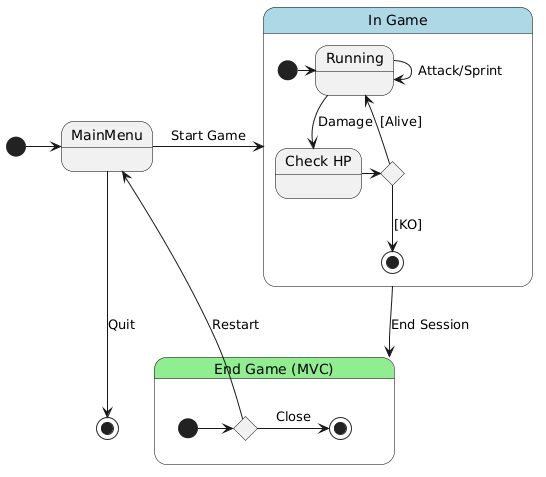
\includegraphics[width=0.6\linewidth]{ActDiag.png}
    \caption{Activity Diagram}
    \label{fig:Activity Diagram} % Serve per fare riferimenti nel testo
\end{figure}

\section*{Descrizione}

Il diagramma illustra gli stati principali dell'applicazione e le transizioni che regolano l'esperienza utente, dal lancio alla chiusura del software:

\begin{small}
\begin{itemize}[leftmargin=*, noitemsep, topsep=0pt]
    \item \textbf{Gestione Menu:} Il sistema inizia nel \texttt{MainMenu}, fungendo da snodo principale per l'avvio del gameplay o l'uscita definitiva dall'applicazione.
    
    \item \textbf{Logica di Gameplay (In Game):} Rappresenta il nucleo interattivo. Lo stato \texttt{Running} gestisce le azioni continue (attacco/sprint). Qualsiasi danno subito innesca un passaggio allo stato di verifica (\texttt{CheckStatus}), dove un nodo decisionale (\texttt{choice}) determina se ripristinare il controllo al giocatore o terminare la sessione in caso di sconfitta o vittoria.
    
    \item \textbf{Ciclo Post-Partita (End Game):} Una volta conclusa la sessione di gioco, il sistema passa alla schermata di \texttt{End Game}. Qui l'utente può scegliere, tramite un punto di decisione, se reinizializzare il ciclo tornando al \texttt{MainMenu} o chiudere l'applicazione.
\end{itemize}

\noindent \textit{Il diagramma garantisce la corretta gestione del ciclo di vita del gioco, separando nettamente la fase di input attivo dalla gestione dei risultati e dei menu.}
\end{small}


\clearpage
%----------------------------------------------------------------------
\section{UML -- Class Diagram}
%----------------------------------------------------------------------
\begin{figure}[htbp]
    \centering % Centra l'immagine nella pagina
    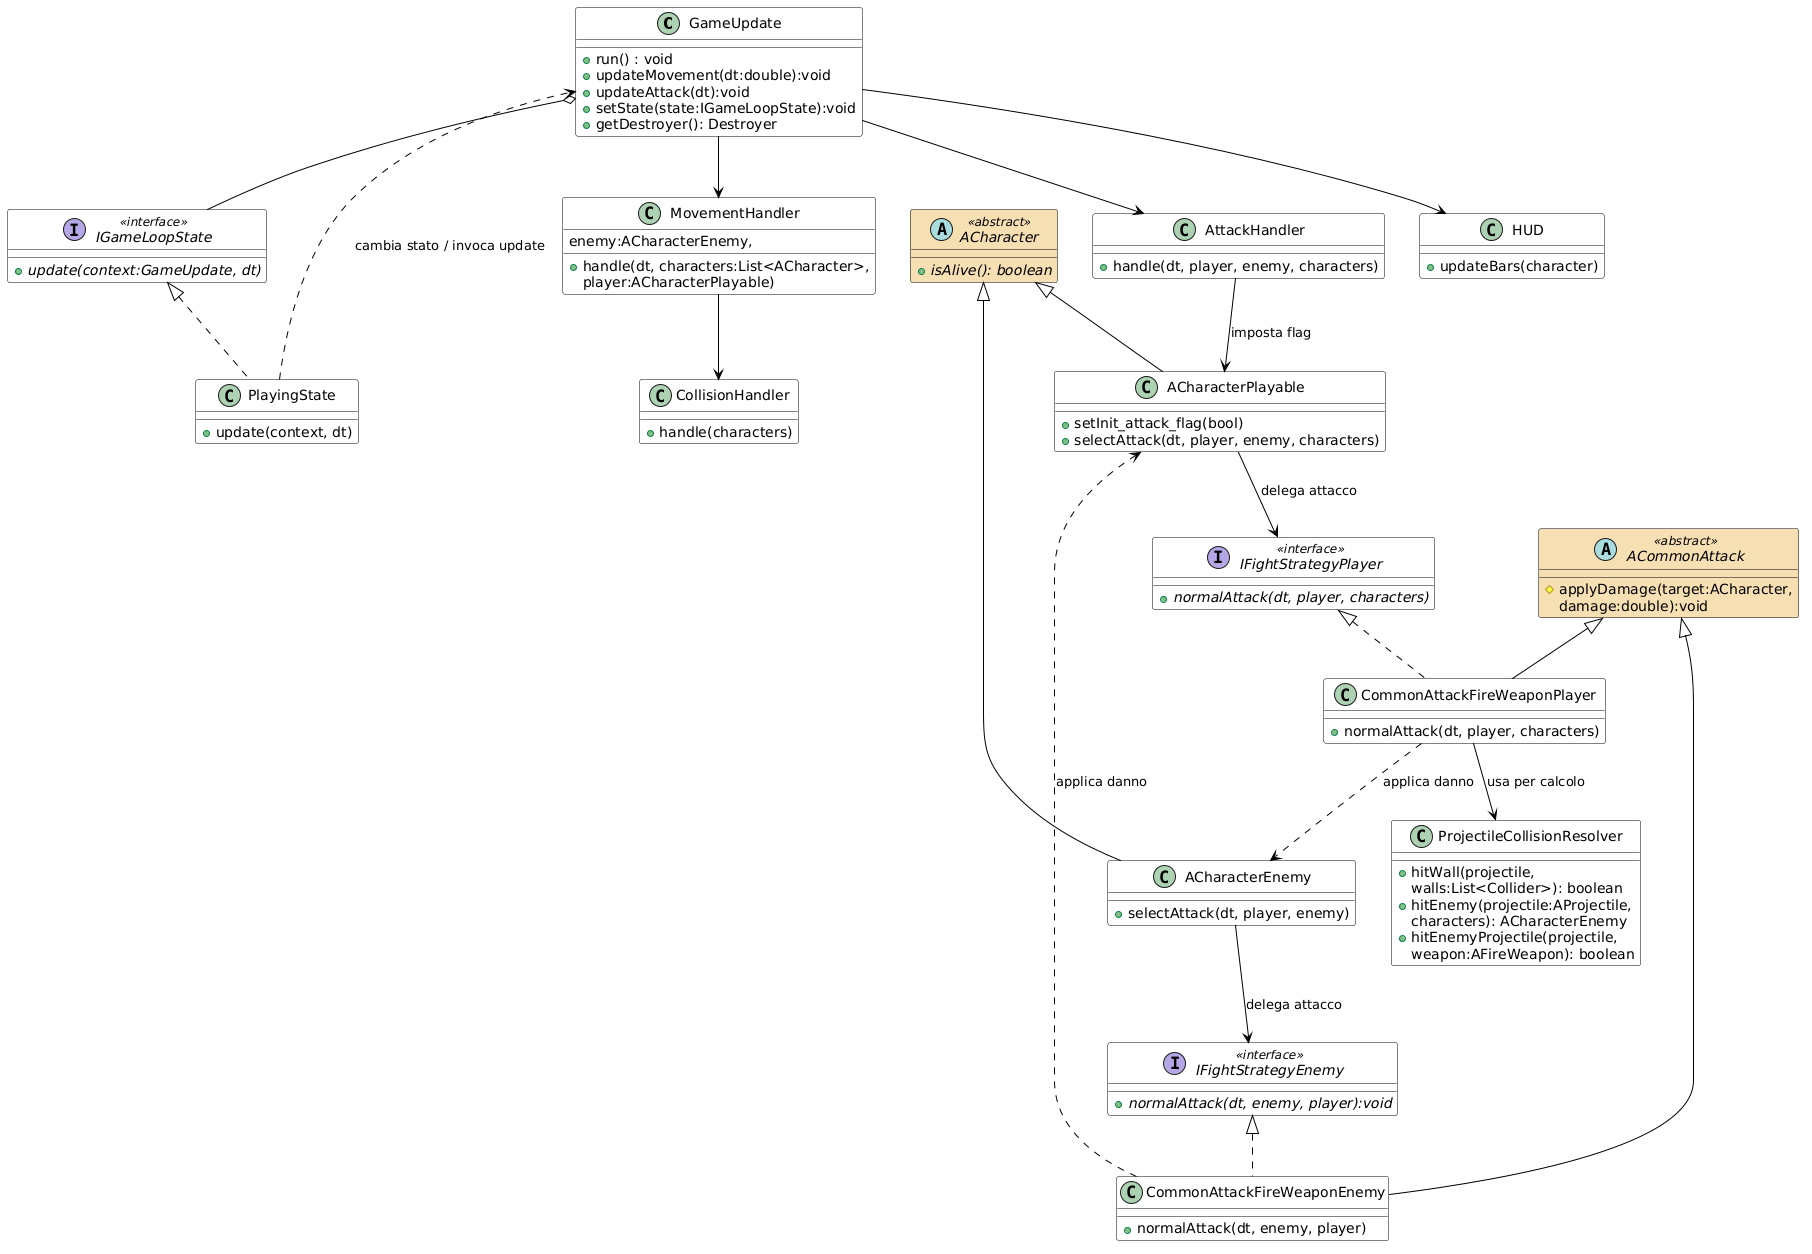
\includegraphics[width=1.0\linewidth]{ClassDiag.png}
    \caption{Class Diagram}
    \label{fig:Class Diagram} % Serve per fare riferimenti nel testo
\end{figure}
\section*{Descrizione}
\begin{small}
L'architettura proposta segue un approccio modulare basato sulla separazione delle responsabilità e sull'estensibilità. I punti cardine sono:

\begin{itemize}[leftmargin=*, noitemsep, topsep=0pt]
    \item \textbf{State Pattern (Core Logic):} Il controllo è delegato a \texttt{PlayingState}. L'uso dell'interfaccia \texttt{State} permette al \texttt{GameUpdate} di cambiare comportamento (es. passare da gioco a menu) senza modificare la struttura del loop principale.
    
    \item \textbf{Disaccoppiamento tramite Handler:} La logica di aggiornamento è suddivisa in componenti specializzati (\texttt{MovementHandler}, \texttt{AttackHandler}). Il \texttt{MovementHandler} delega ulteriormente la fisica al \texttt{CollisionHandler}, isolando i calcoli di movimento dalle verifiche di collisione.
    
    \item \textbf{Strategy Pattern (Combattimento):} Le strategie d'attacco (\texttt{IFightStrategy}) sono separate dalle classi dei personaggi. Questo permette di variare le meccaniche di attacco (es. proiettili o mischia) a runtime semplicemente scambiando l'implementazione della strategia, garantendo elevata flessibilità.
    
    \item \textbf{Utility e UI:} La classe \texttt{ProjectileCollisionResolver} centralizza la logica geometrica dei proiettili, riducendo la ridondanza. L'interfaccia utente (\texttt{HUD}) è mantenuta passiva, aggiornata direttamente dal ciclo di gioco per garantire la coerenza dei dati visualizzati.
\end{itemize}

\noindent \textit{Il sistema applica rigorosamente i principi SOLID, facilitando l'aggiunta di nuovi contenuti (nemici, armi o stati) senza alterare il codice preesistente.}
\end{small}


\clearpage
\section{UML -- Sequence Diagram}
\begin{figure}[htbp]
    \centering % Centra l'immagine nella pagina
    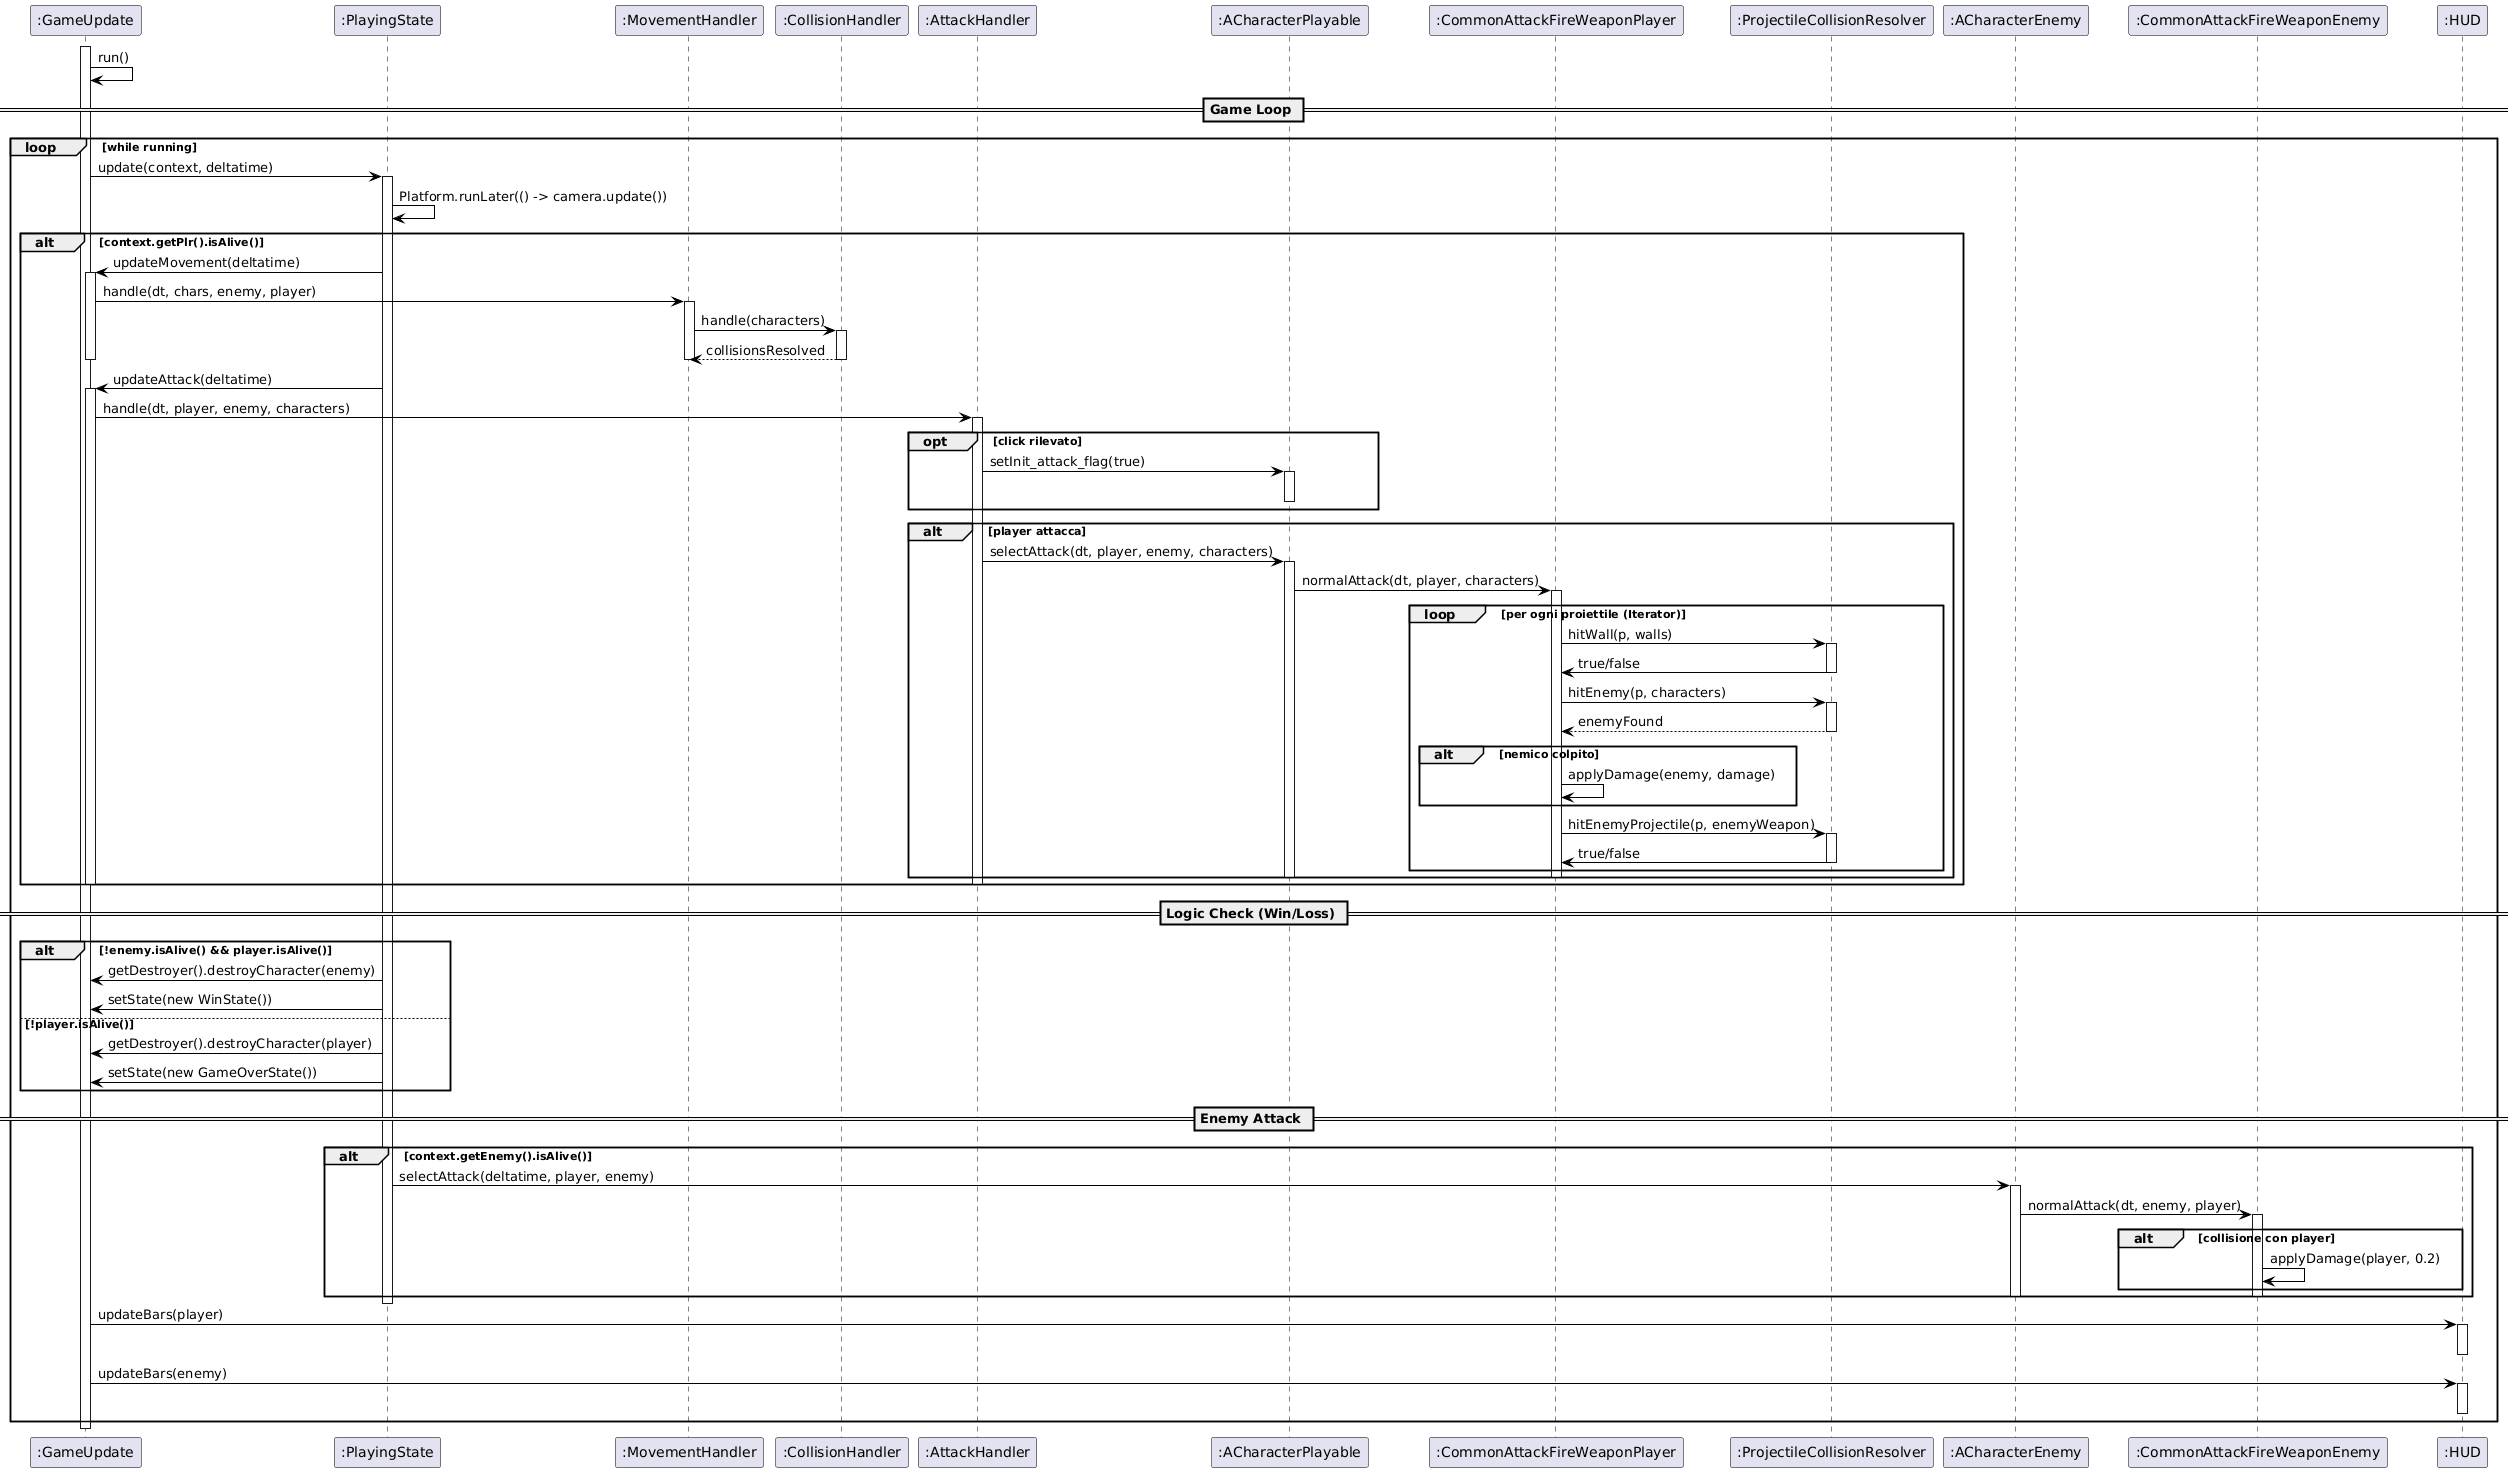
\includegraphics[width=1.15\linewidth]{SeqDiag.png}
    \caption{Sequence Diagram}
    \label{fig:Sequence Diagram} % Serve per fare riferimenti nel testo
\end{figure}

\section*{Descrizione}
\begin{small}
Il diagramma illustra il flusso iterativo del \texttt{GameLoop}, orchestrato dalla classe \texttt{GameUpdate} che delega l'aggiornamento della logica allo stato corrente (\texttt{PlayingState}). Il processo si divide in quattro fasi principali:

\begin{itemize}[leftmargin=*, noitemsep, topsep=0pt]
    \item \textbf{Gestione Fisica e Input:} Se il giocatore è in vita, vengono invocati i gestori del movimento (\texttt{MovementHandler}) e delle collisioni. Successivamente, l'\texttt{AttackHandler} processa l'input (click del mouse) per inizializzare o continuare la sequenza di attacco.
    
    \item \textbf{Risoluzione dei Combattimenti:} La logica degli attacchi è delegata a classi strategia (\texttt{CAP} per il player, \texttt{CAE} per il nemico). Per il giocatore, un iteratore gestisce ogni proiettile attivo, verificando tramite il \texttt{PCR} (Collision Resolver) impatti con muri, nemici o proiettili avversari e applicando il relativo danno.
    
    \item \textbf{Verifica delle Condizioni di Terminazione:} Al termine di ogni ciclo, lo stato controlla la vitalità dei personaggi. Se uno dei due soccombe, viene invocato il \texttt{Destroyer} per la rimozione del nodo grafico e viene eseguito il cambio di stato verso \texttt{WinState} o \texttt{GameOverState}.
    
    \item \textbf{Aggiornamento Grafico:} L'ultima fase del ciclo prevede l'aggiornamento delle barre della salute nell'\texttt{HUD} per entrambi i personaggi, garantendo il feedback immediato all'utente.
\end{itemize}

\noindent \textit{Nota tecnica: L'uso di \texttt{Platform.runLater} per l'aggiornamento della camera indica una gestione asincrona del rendering rispetto alla logica di gioco.}
\end{small}


\end{document}